\begin{figure}[H]
	\centering
	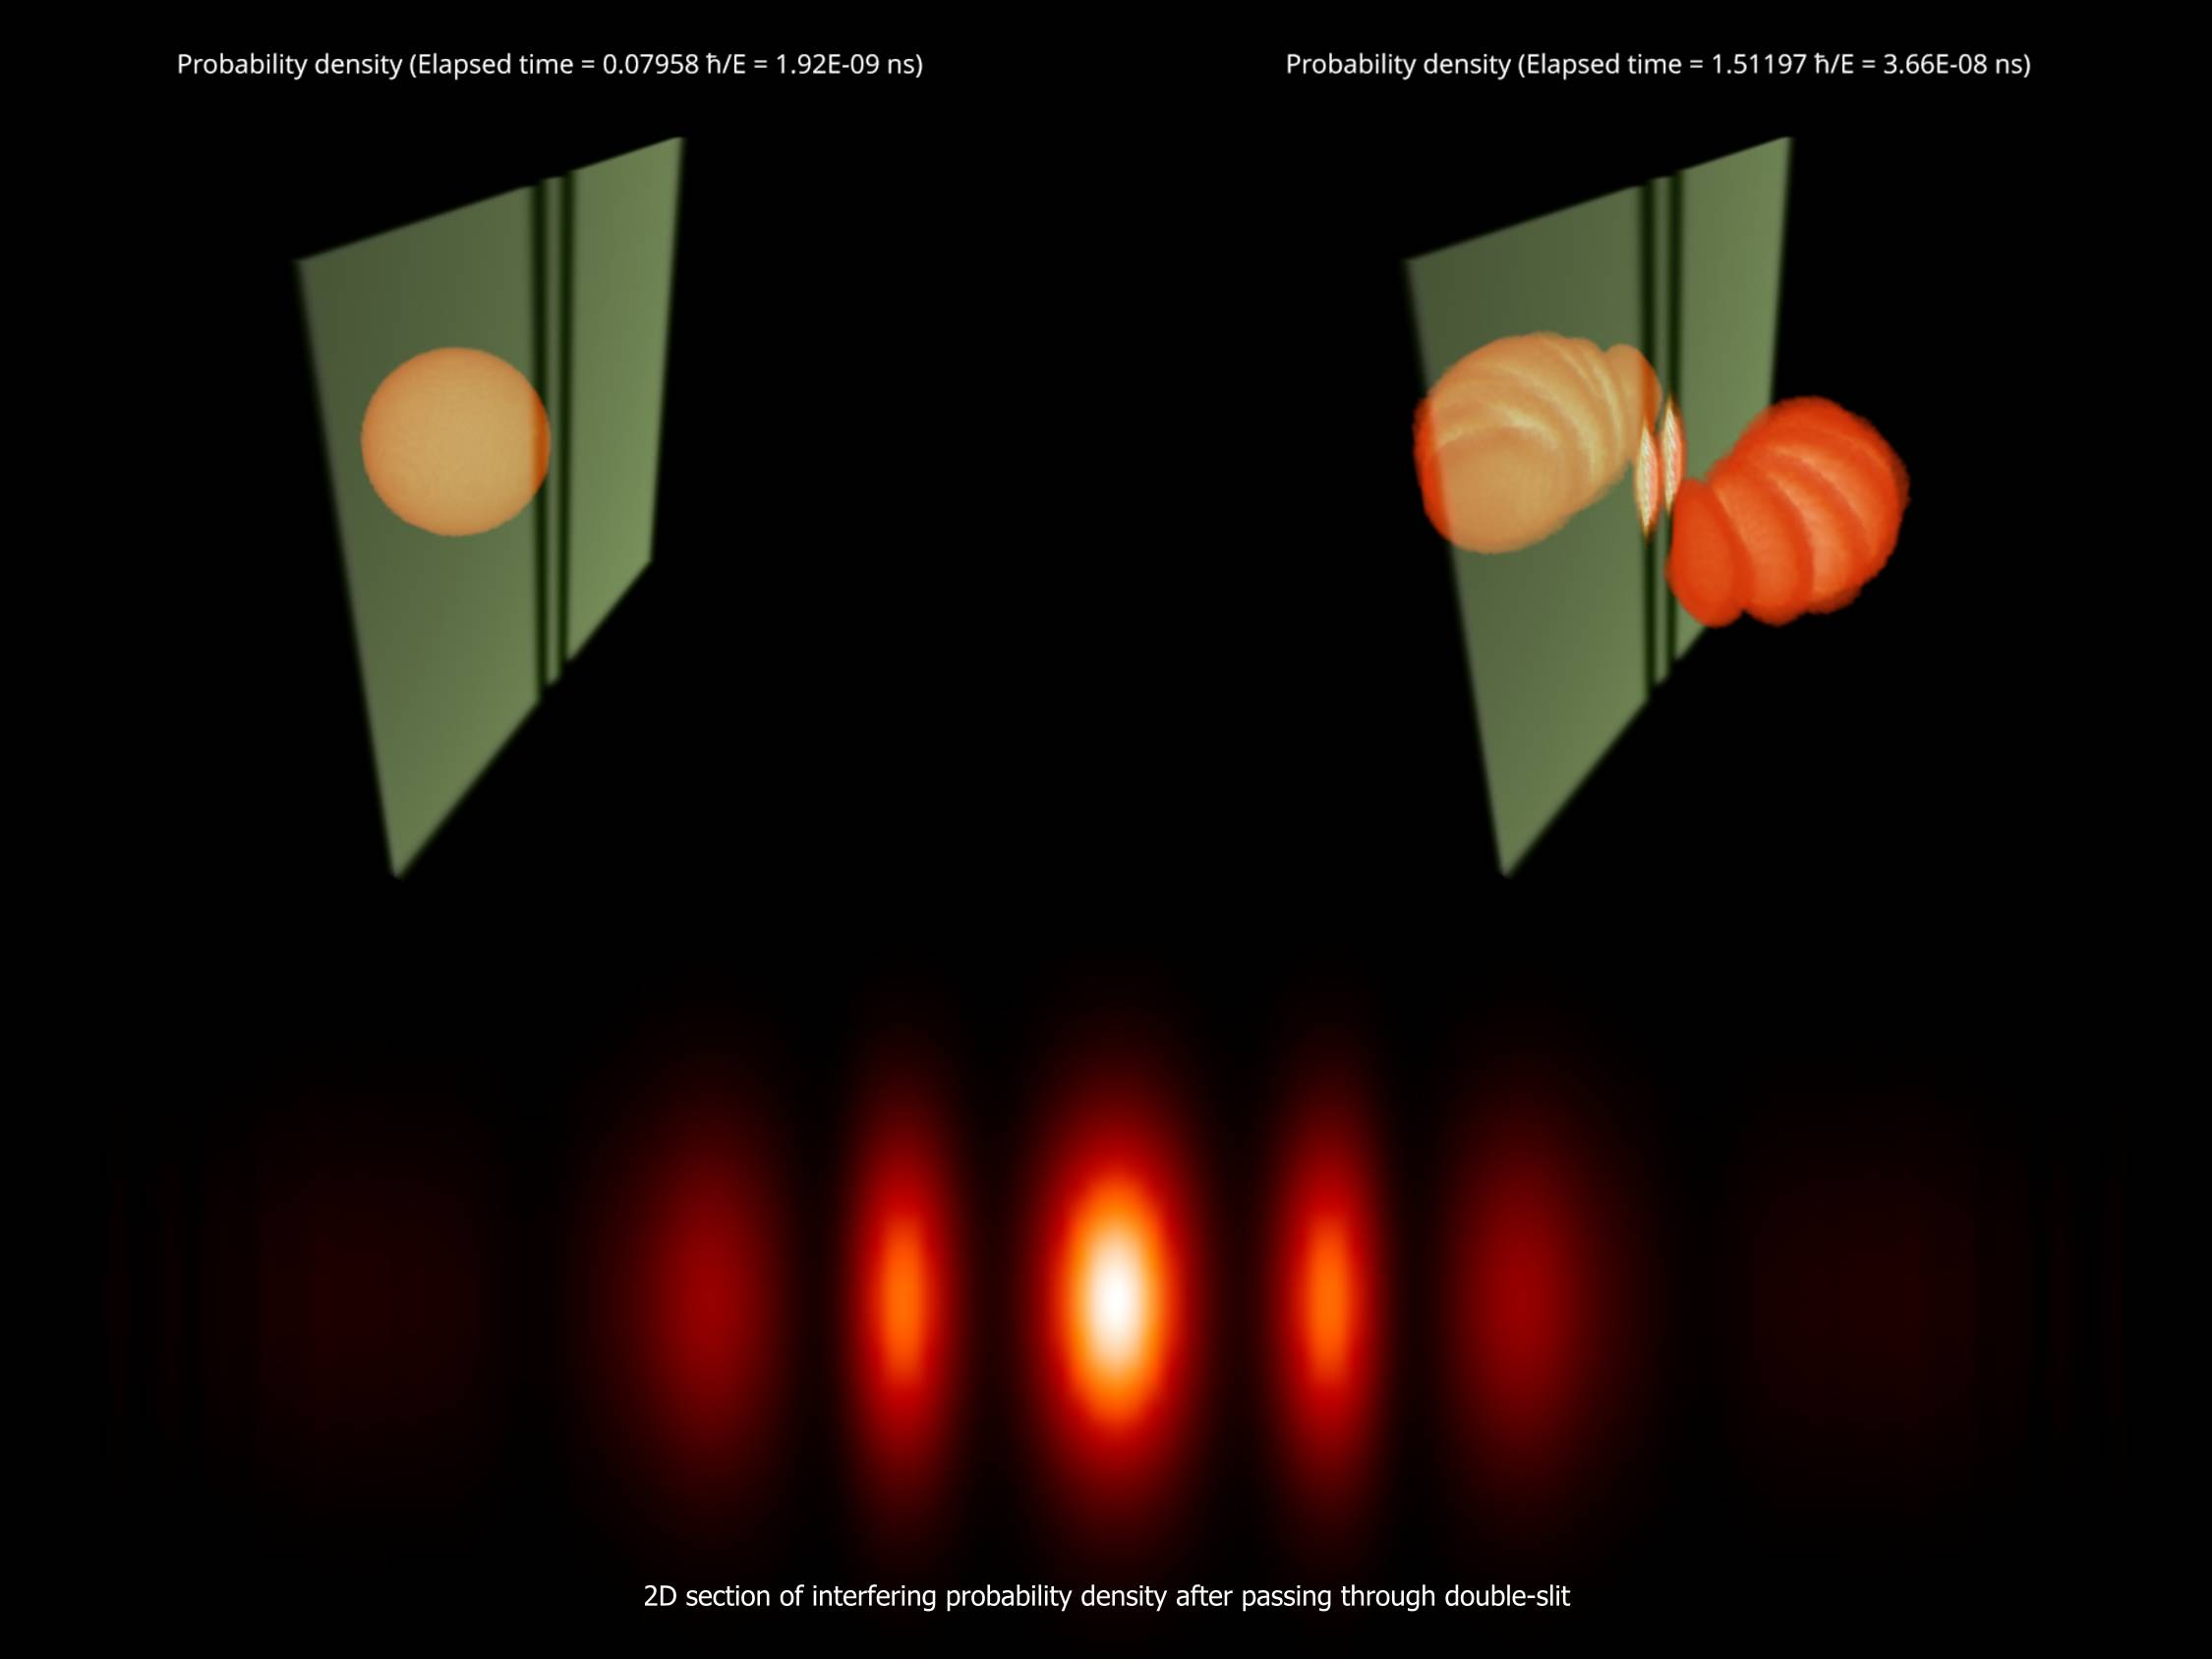
\includegraphics[width=0.5\textwidth]{"figures/preview_image.jpeg"}
	\caption{Wave packet going through double slit.}
	\label{fig:penetrating_potential}
\end{figure}

\section*{Abstract}

In quantum mechanics, the wave function describes the state of a physical system. In the non-relativistic case, the time evolution of the wave function is described by the time-dependent Schrödinger equation. In 1982, D Kosloff and R Kosloff proposed a method \cite{KOSLOFF198335} to solve the time-dependent Schrödinger equation efficiently using Fourier transformation. In 2020, Géza István Márk published a paper \cite{mark2020webschrodinger} describing a computer program for the interactive solution of the time-dependent and stationary two-dimensional (2D) Schrödinger equation. Some details of quantum phenomena are only observable by calculating with all three spatial dimensions. We found it worth stepping out from the two-dimensional plane and investigating these phenomena in three dimensions. We implemented the said method for the three-dimensional case to simulate the time evolution of the wave function. We used our implementation to simulate typical quantum phenomena using wave packet dynamics. First, we tried the method on analytically describable cases, such as the simulation of the double-slit experiment, then we investigated the operation of flash memory. We used raytraced volumetric visualization to render the resulting probability density. In our work, we introduce the basics of wave packet dynamics in quantum mechanics. We describe the method in use in detail and showcase our simulation results.\\
For further information and animations please visite\\ \url{https://zoltansimon.info/src/content/research/wavepacketsim.html}

\selectlanguage{magyar}
\section*{Kivonat}

A kvantummechanikában a hullámfüggvény írja le egy fizikai rendszer állapotát. Nemrelativisztikus esetben a hullámfüggvény időbeli fejlődését az időfüggő Schrödinger-egyenlet határozza meg. 1982-ben D Kosloff és R Kosloff közölt egy módszert \cite{KOSLOFF198335} az időfüggő Schrödinger-egyenlet hatékony megoldására Fourier-transzformáció felhasználásával. 2020-ban Márk Géza István cikkében \cite{mark2020webschrodinger} bemutatott egy interaktív szá\-mí\-tó\-gé\-pes programot az időfüggő és a stacionárius kétdimenziós Schrödinger-egyenlet megoldására. A kvantumos jelenségek bizonyos részletei csak mindhárom térdimenzióval számolva figyelhetők meg. Érdemesnek tartottuk a síkból kilépve, térben is megvizsgálni ezeket a jelenségeket. Munkánkban háromdimenziós esetre implementáltuk az említett módszert, hogy szimuláljuk a hullámfüggvény időbeli fejlődését. Hullámcsomag-dinamikát használva kipróbáltuk több jellegzetes kvantumos jelenség szimulációját. A módszert először analitikusan kezelhető esetekre teszteltük, például a kétréses kísérlet szimulációjára, ezután megvizsgáltuk a flash memória cella működését. A szimuláció kimeneteként előálló valószínűségi sűrűséget sugárkövetéses térfogati megjelenítéssel ábrázoltuk. Dolgozatunkban ismertetjük a kvantummechanikai hullámcsomag-dinamika alapjait. Részletesen leírjuk a használt eljárást, és bemutatjuk a szimulációnk eredményeit.\\
További információ és animációk találhatóak a\\ \url{https://zoltansimon.info/src/content/research/wavepacketsim.html} webcímen.

\selectlanguage{english}
